% !TEX root = main.tex
%////////////////////////////////////////////////////////
\begin{center}
\section*{\kintou{2.5zw}{付録}}                      %% ここに番号をつけない
\vspace*{-2zh}
\end{center}
\addcontentsline{toc}{section}{付録} %% 目次に番号をつけない
\appendix

\setcounter{equation}{0}
\setcounter{figure}{0}
\setcounter{table}{0}

\makeatletter
     \renewcommand{\theequation}{%
          A.\arabic{equation}}
     \@addtoreset{equation}{section}
\makeatother

\makeatletter
     \renewcommand{\thetable}{%
          A.\arabic{table}}
     \@addtoreset{table}{section}
\makeatother

\makeatletter
     \renewcommand{\thefigure}{%
          A.\arabic{figure}}
     \@addtoreset{figure}{section}
\makeatother

% ================================================
\makeatletter
     \renewcommand{\thesubsection}{%
          A.\arabic{subsection}}
     \@addtoreset{subsection}{section}
\makeatother

\makeatletter
     \renewcommand{\thesubsubsection}{%
          A.\arabic{subsection}.\arabic{subsubsection}}
     \@addtoreset{subsubsection}{section}
\makeatother

% ================================================
\makeatletter
     \renewcommand{\thetheorem}{%
          A.\arabic{theorem}}
     \@addtoreset{theorem}{section}
\makeatother

\makeatletter
     \renewcommand{\thedefinition}{%
          A.\arabic{definition}}
     \@addtoreset{definition}{section}
\makeatother

\makeatletter
     \renewcommand{\thelemma}{%
          A.\arabic{lemma}}
     \@addtoreset{lemma}{section}
\makeatother

\makeatletter
     \renewcommand{\thelstlisting}{%
          {\bf{A.\arabic{lstlisting}}}}
     \@addtoreset{lstlisting}{section}
\makeatother






%////////////////////////////////////////////////////////

\subsection{Solidedgeを用いたモデルの作製と3Dプリンターの設定}
 まずSolidedgeを用いて.par形式の3Dパーツを作製し,
.stl形式のファイルに変換する.
そのファイルをスライサーソフトで開く.

 使用した3DプリンターはQIDI~TECH社製のX-PLUS3で,
スライサーソフトにはQIDI~TECH社が提供しているQIDI~Slicer~Ver.1.0.7を用いている.
フィラメントはPLA~Rapidoである.
以下に,.stl形式のファイルをGコードに変換する方法を示す.
上のメニューから.stlファイルを選択し,後述する設定を行った後,スライスを実行する.
最後にGコードをエクスポートして,3Dプリンターで実行すれば印刷が行える.
\begin{figure}[H]
	\centering
		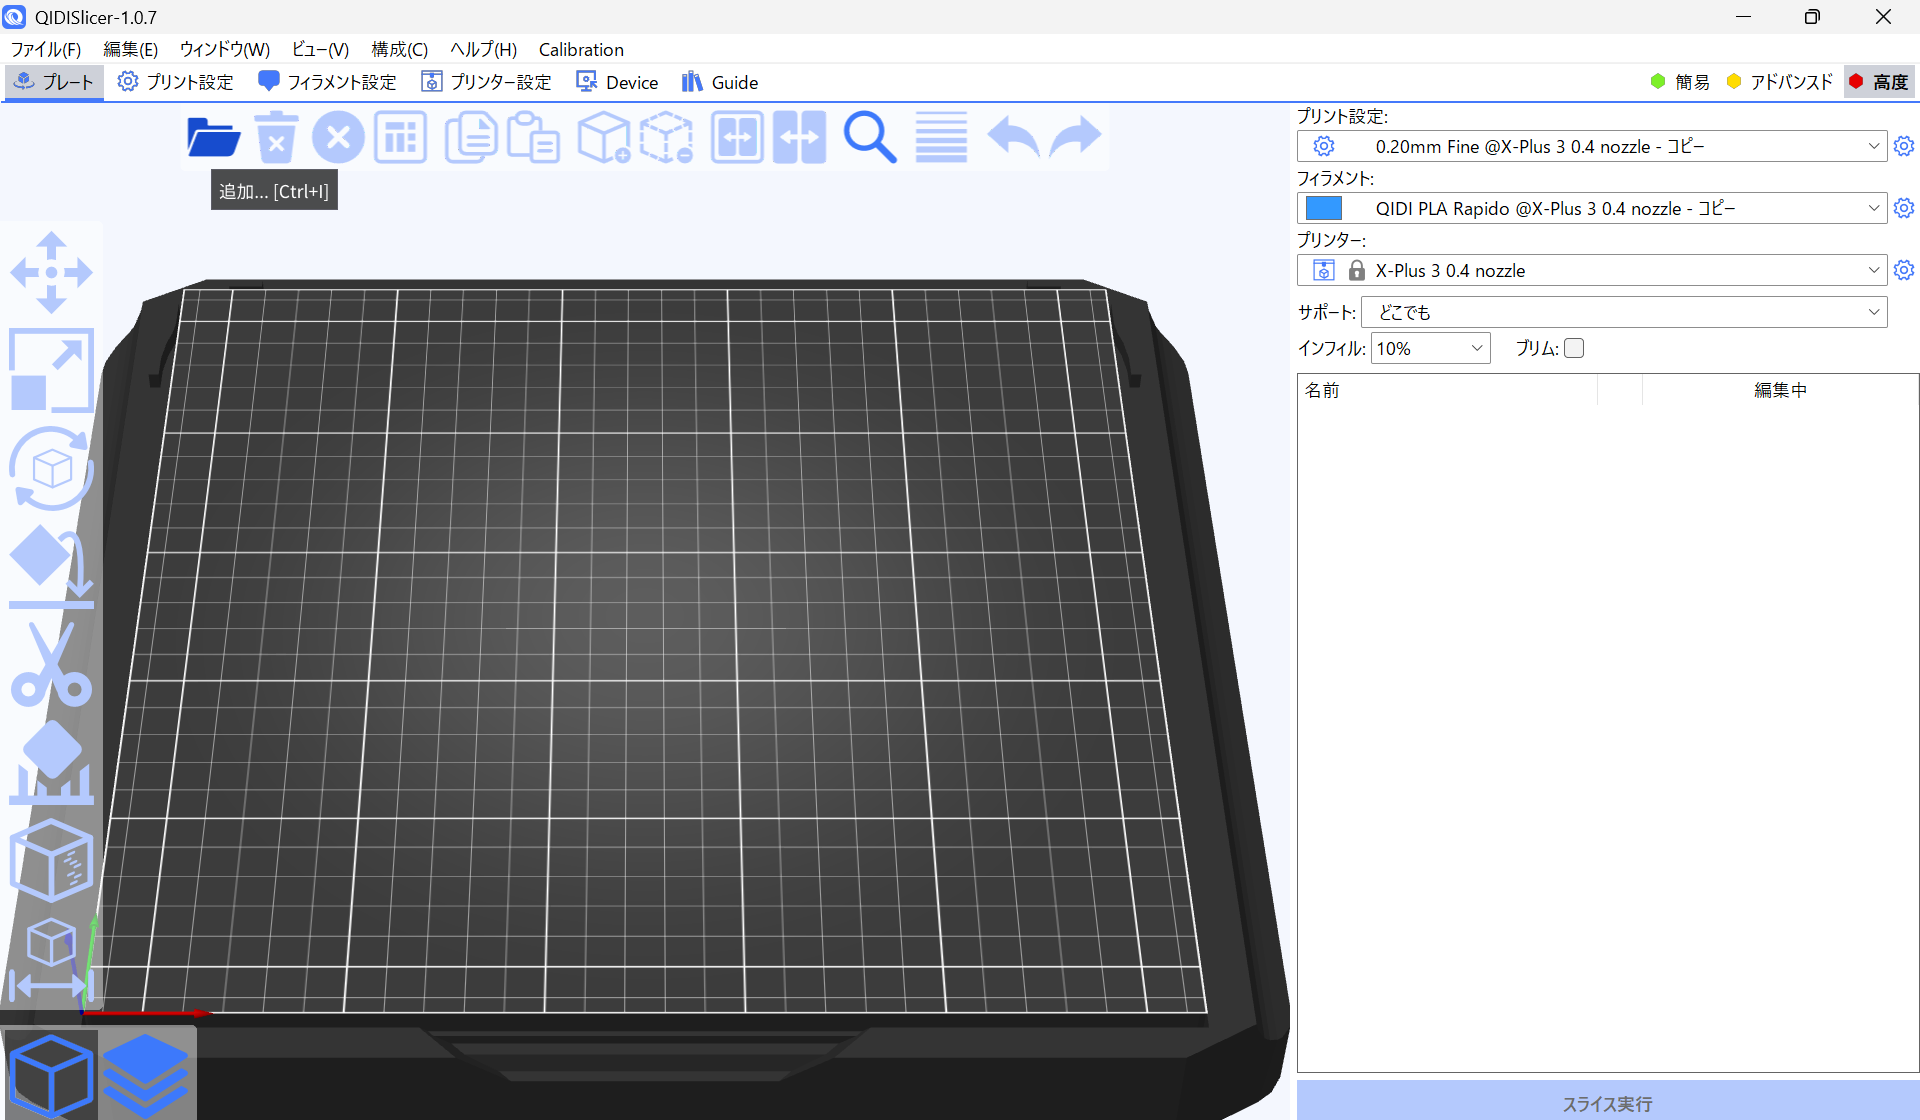
\includegraphics[scale=0.225]{./figure/step1.png}
		\caption{step1}
		\label{fig:step1}
\end{figure}
\begin{figure}[H]
	\centering
		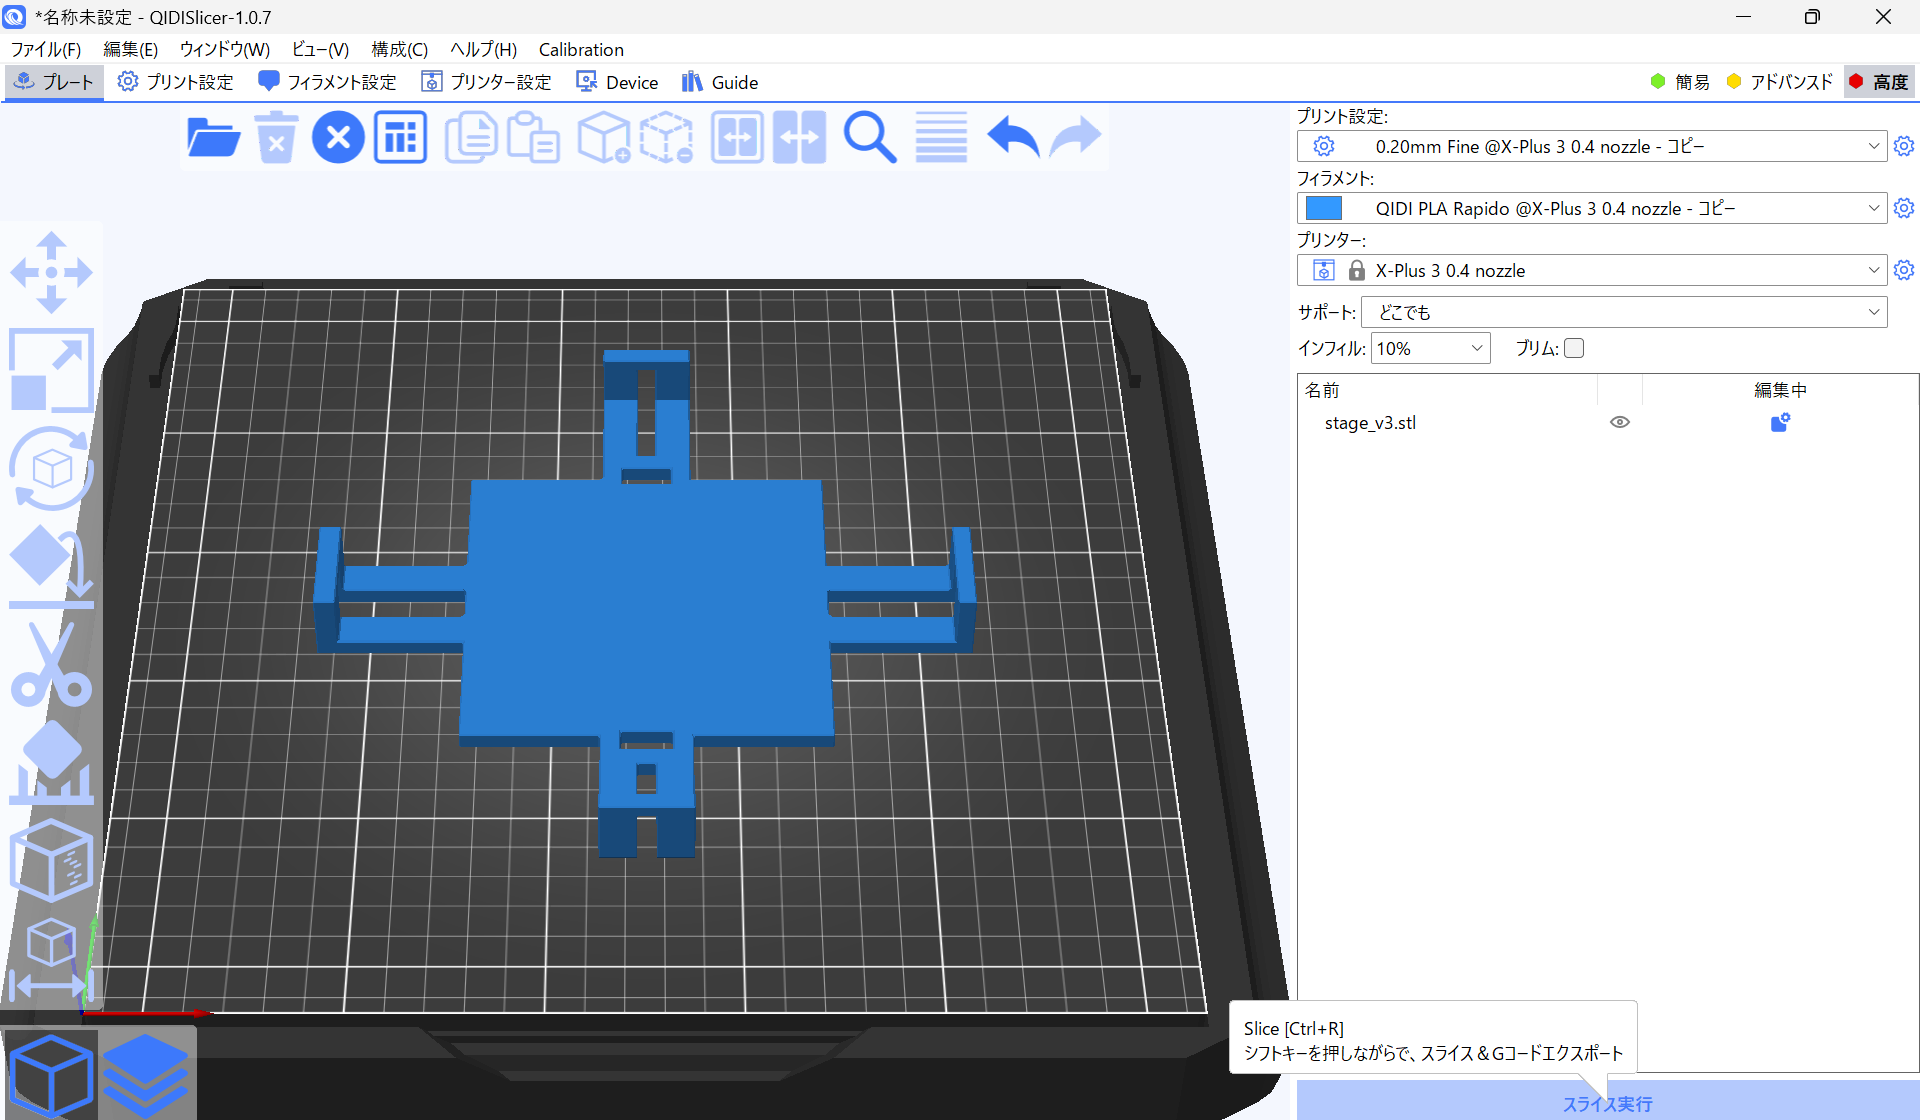
\includegraphics[scale=0.225]{./figure/step2.png}
		\caption{step2}
		\label{fig:step2}
\end{figure}
\begin{figure}[H]
	\centering
		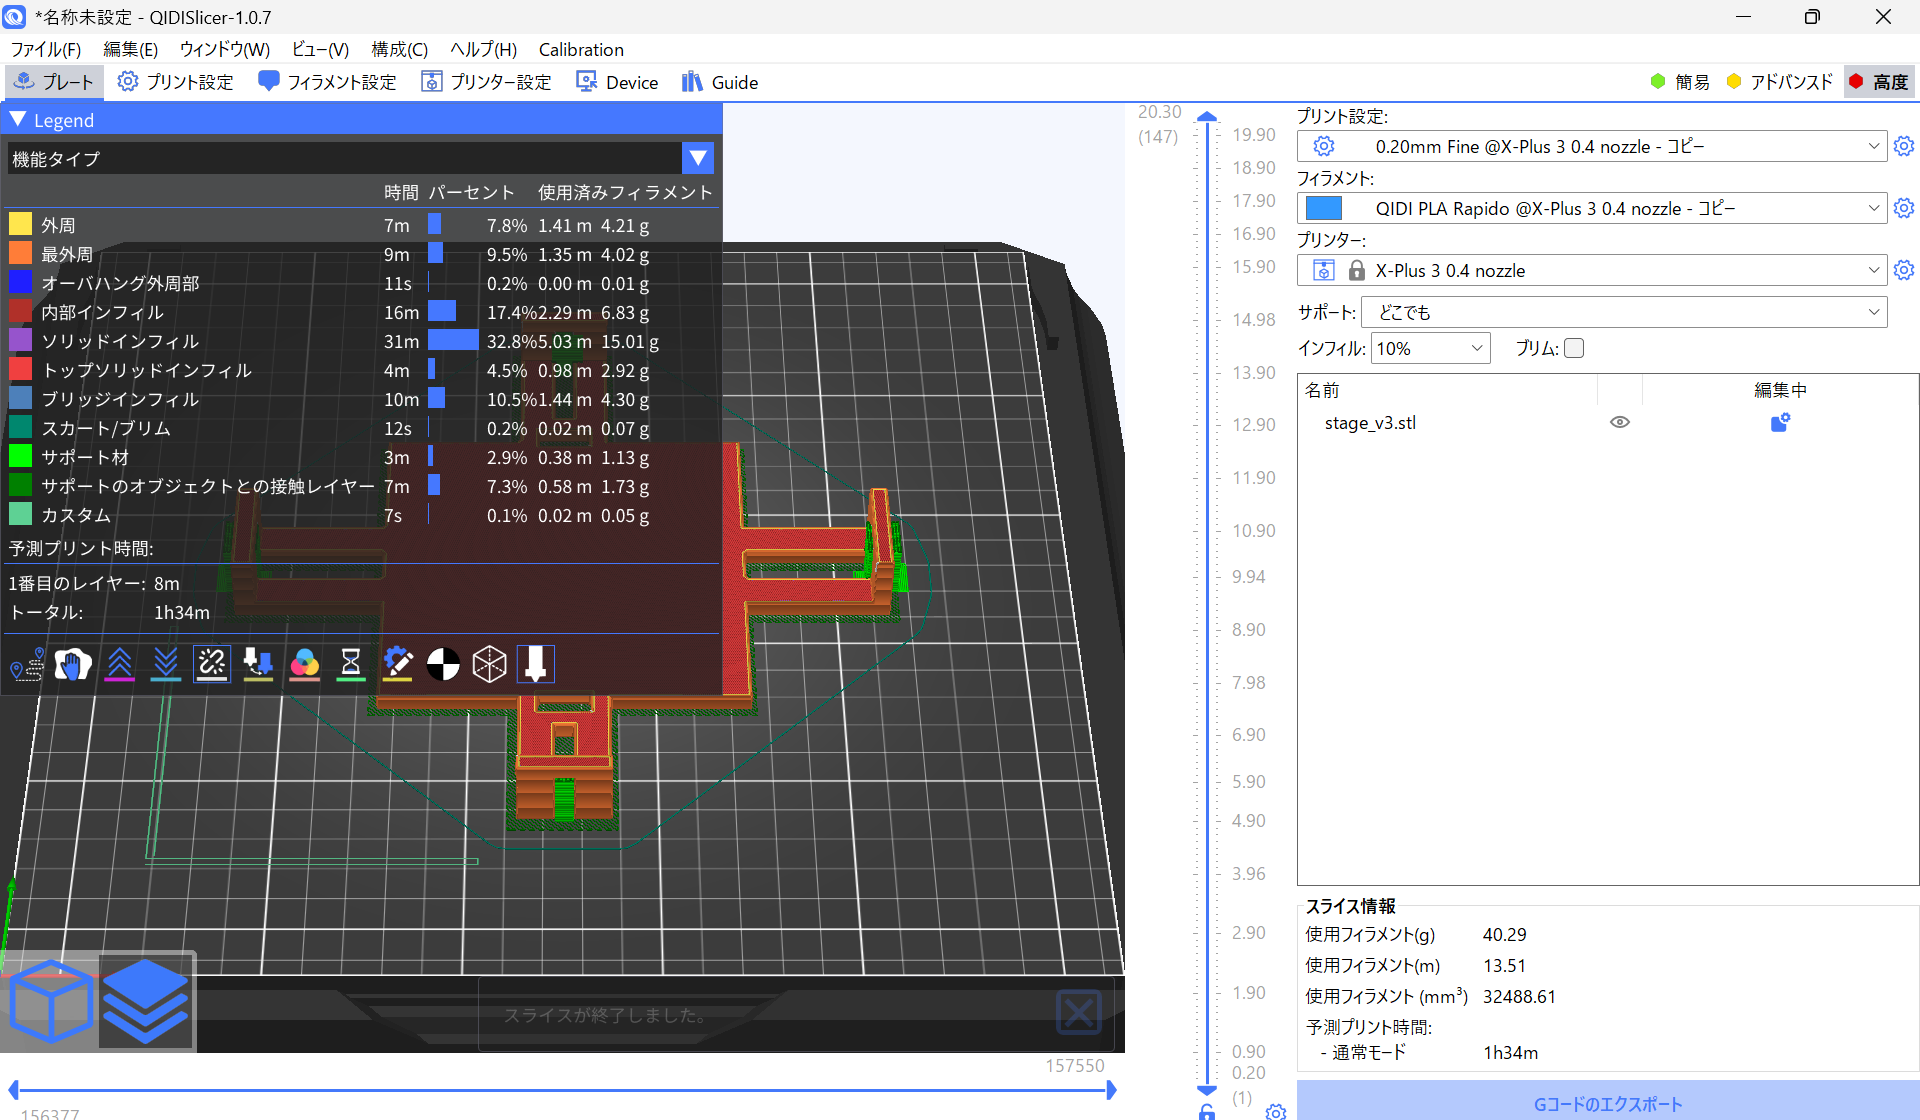
\includegraphics[scale=0.225]{./figure/step3.png}
		\caption{step3}
		\label{fig:step3}
\end{figure}

以下に,デフォルトから変更した設定をスクリーンショットで示す.
変更された設定には青色の錠前マークがついている.

\begin{figure}[H]
	\centering
		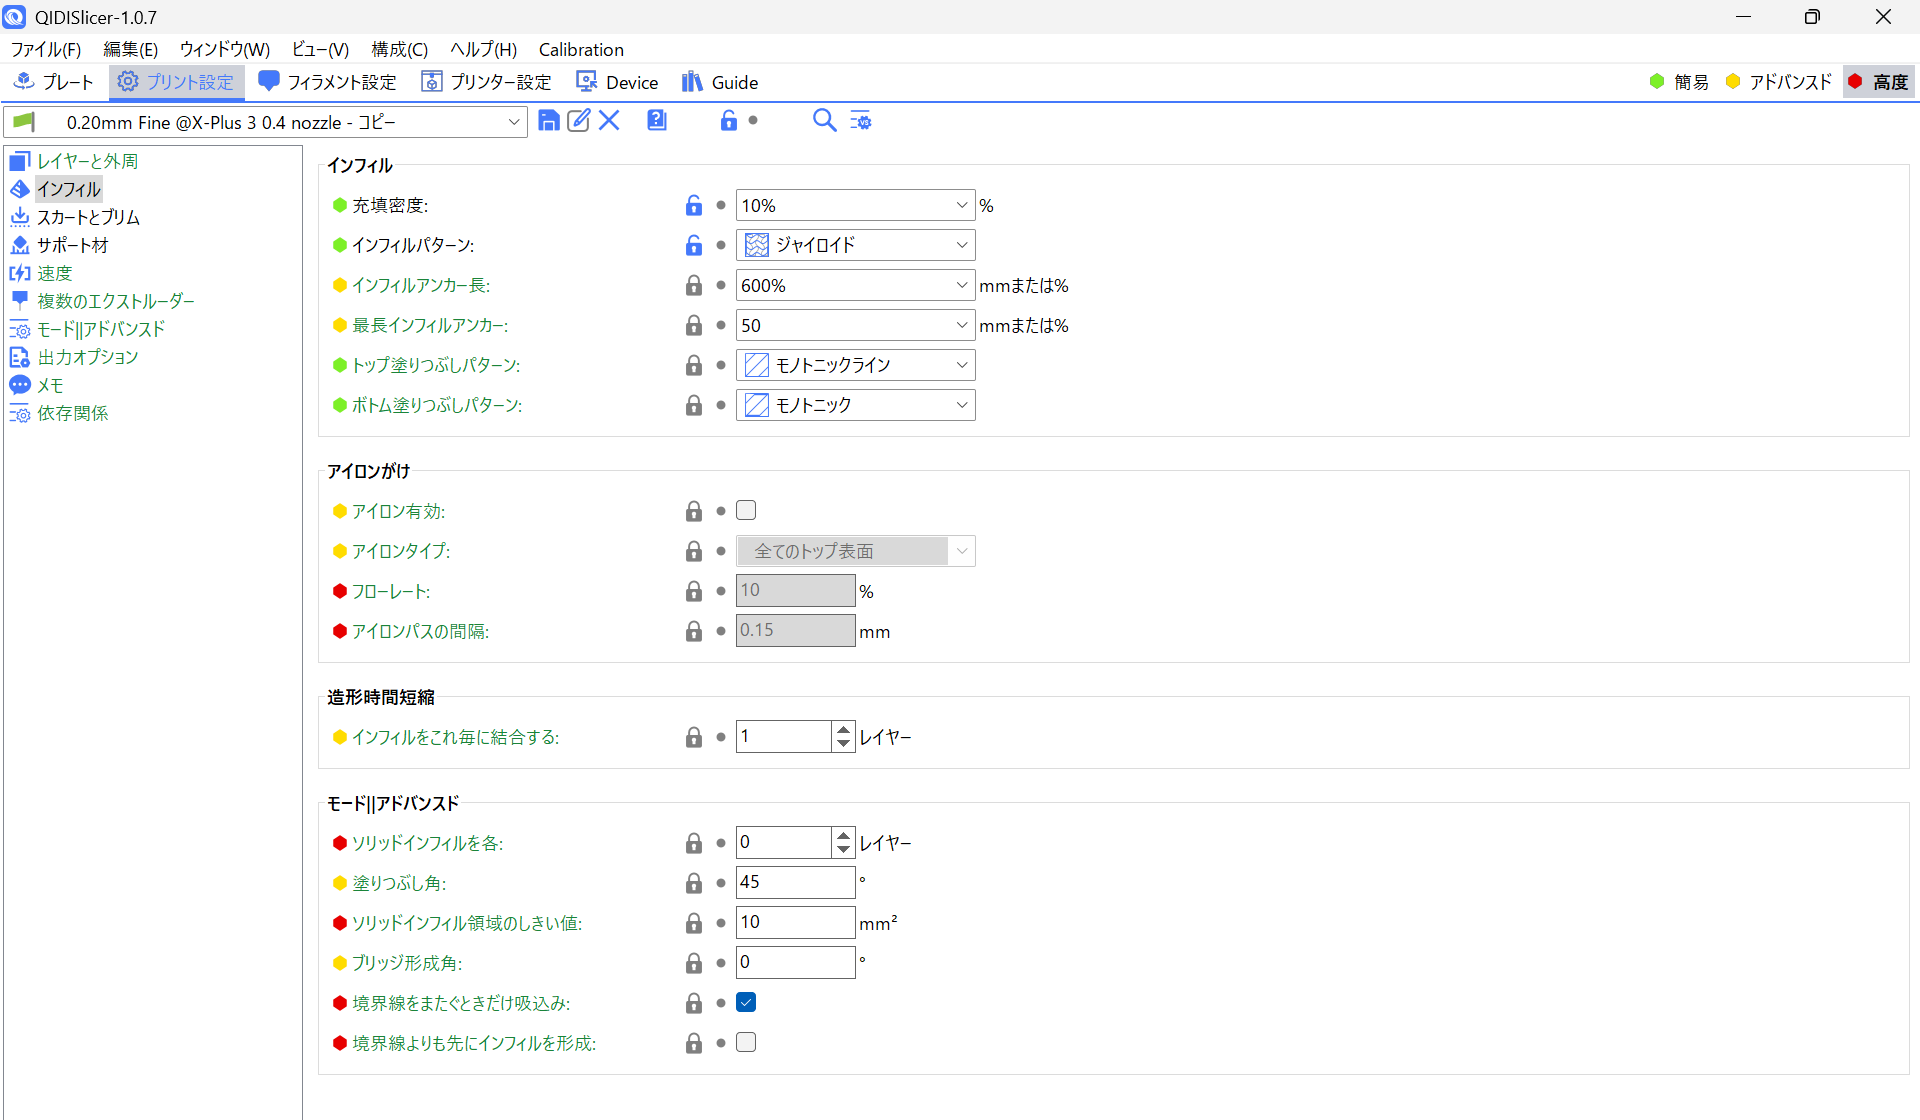
\includegraphics[scale=0.25]{./figure/設定1.png}
		\caption{インフィル}
		\label{fig:slice1}
\end{figure}

\begin{figure}[H]
	\centering
		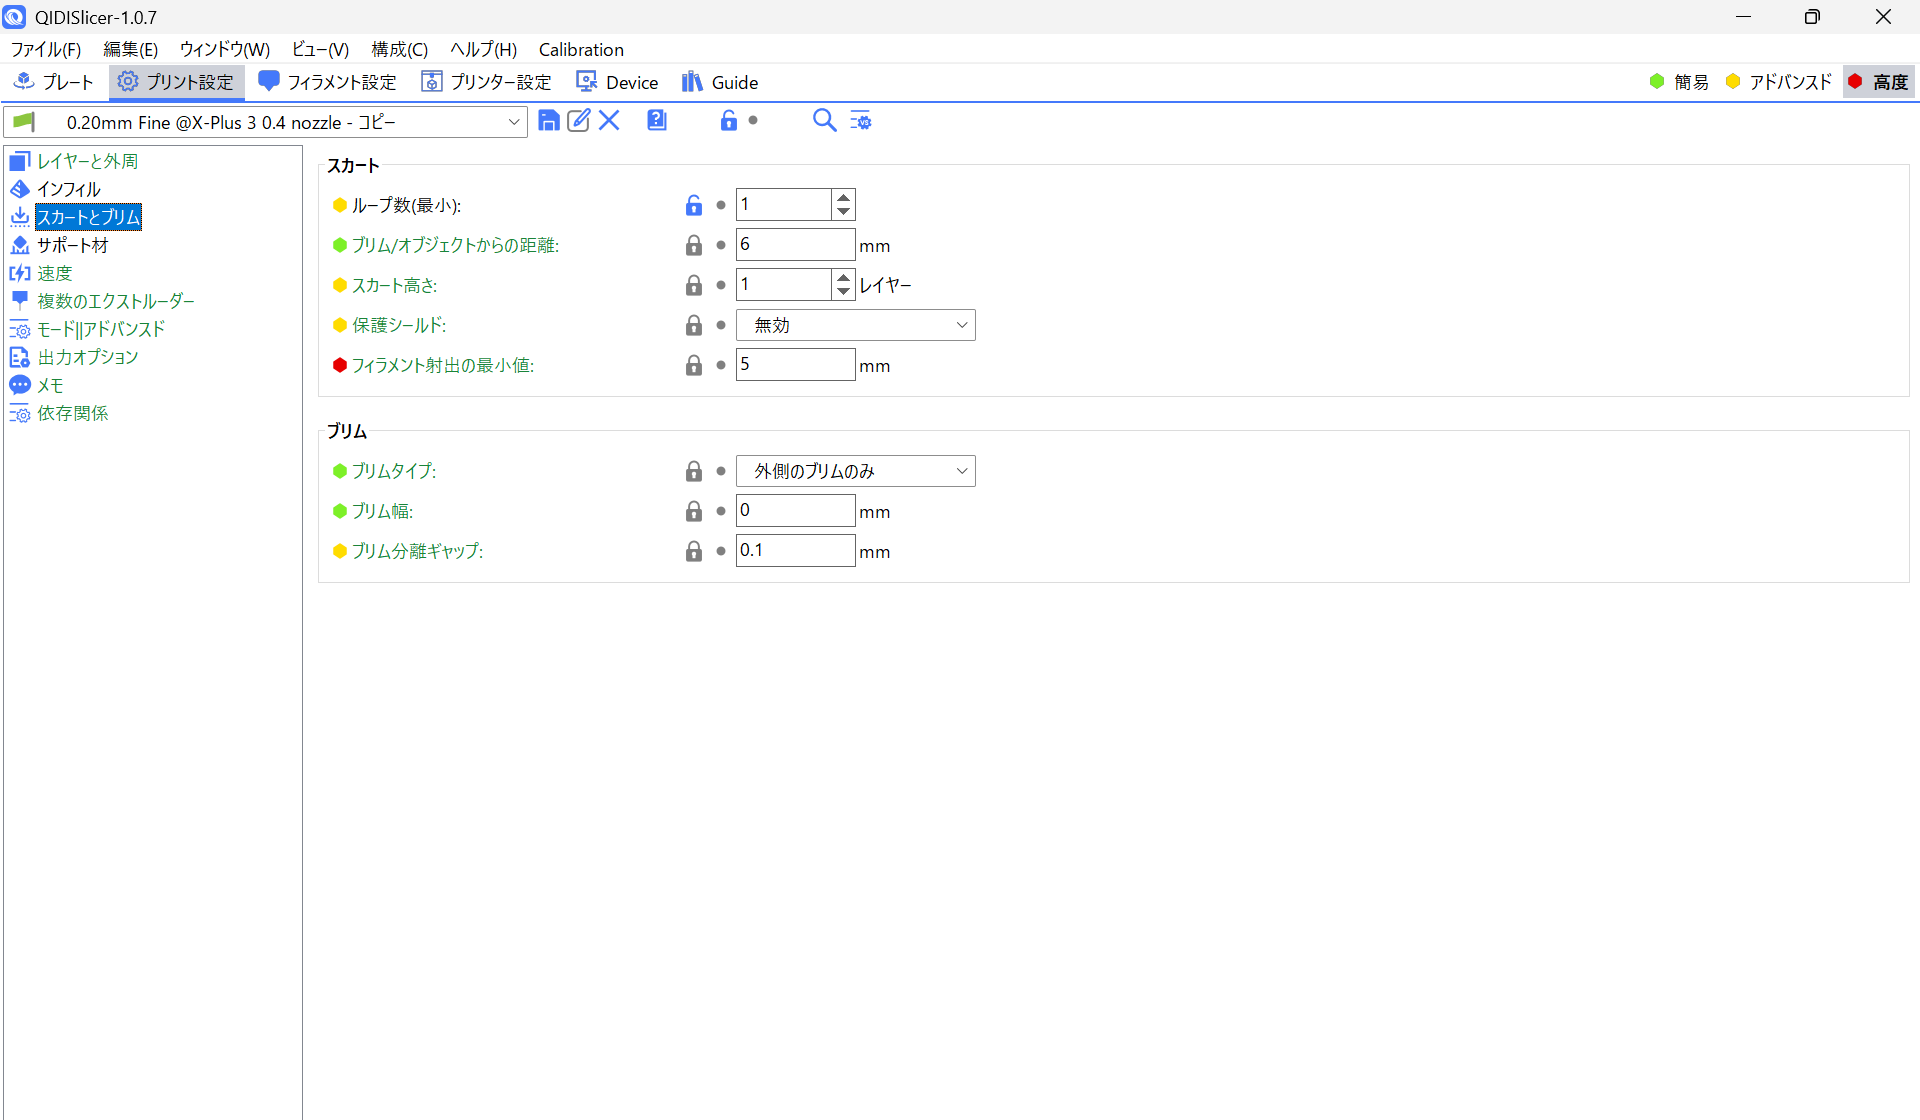
\includegraphics[scale=0.25]{./figure/設定2.png}
		\caption{スカートとプリム}
		\label{fig:slice2}
\end{figure}

\begin{figure}[H]
	\centering
		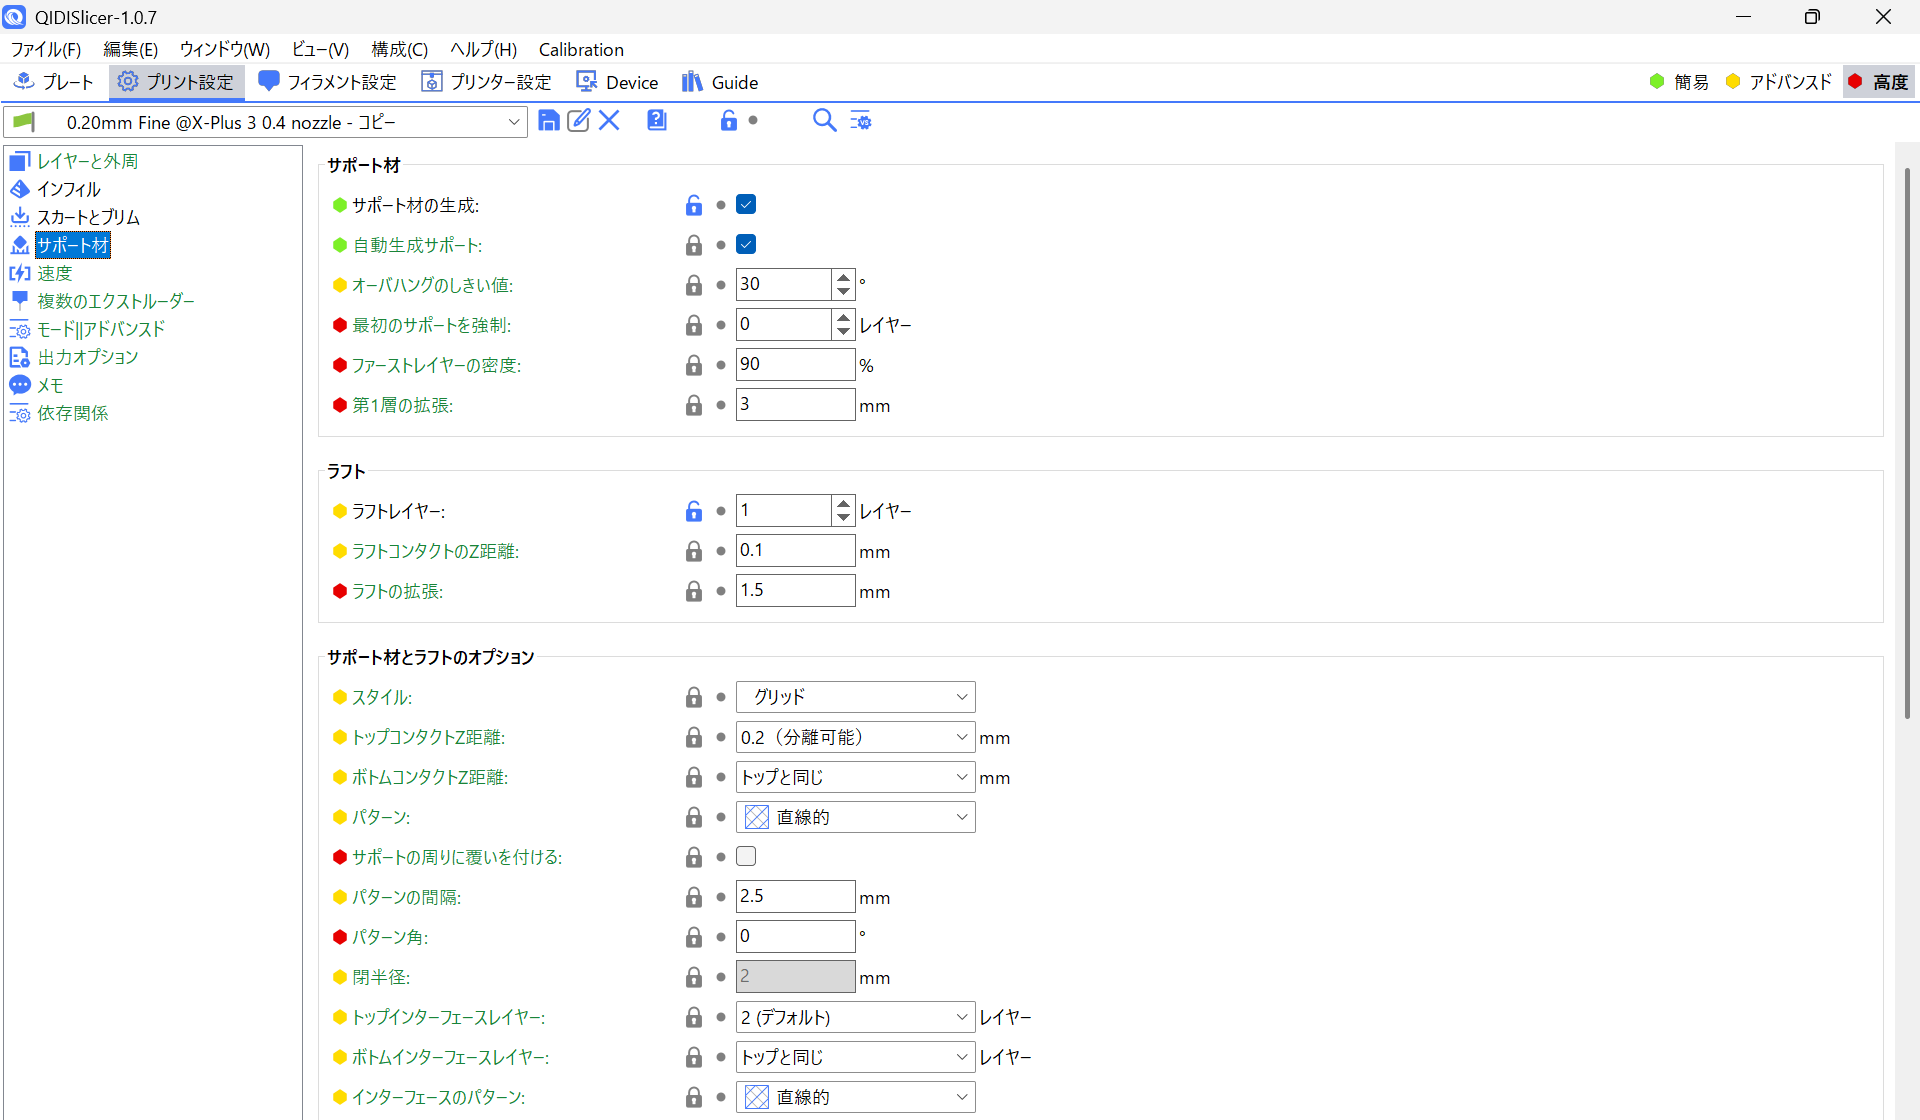
\includegraphics[scale=0.25]{./figure/設定3.png}
		\caption{サポート材}
		\label{fig:slice3}
\end{figure}

\begin{figure}[H]
	\centering
		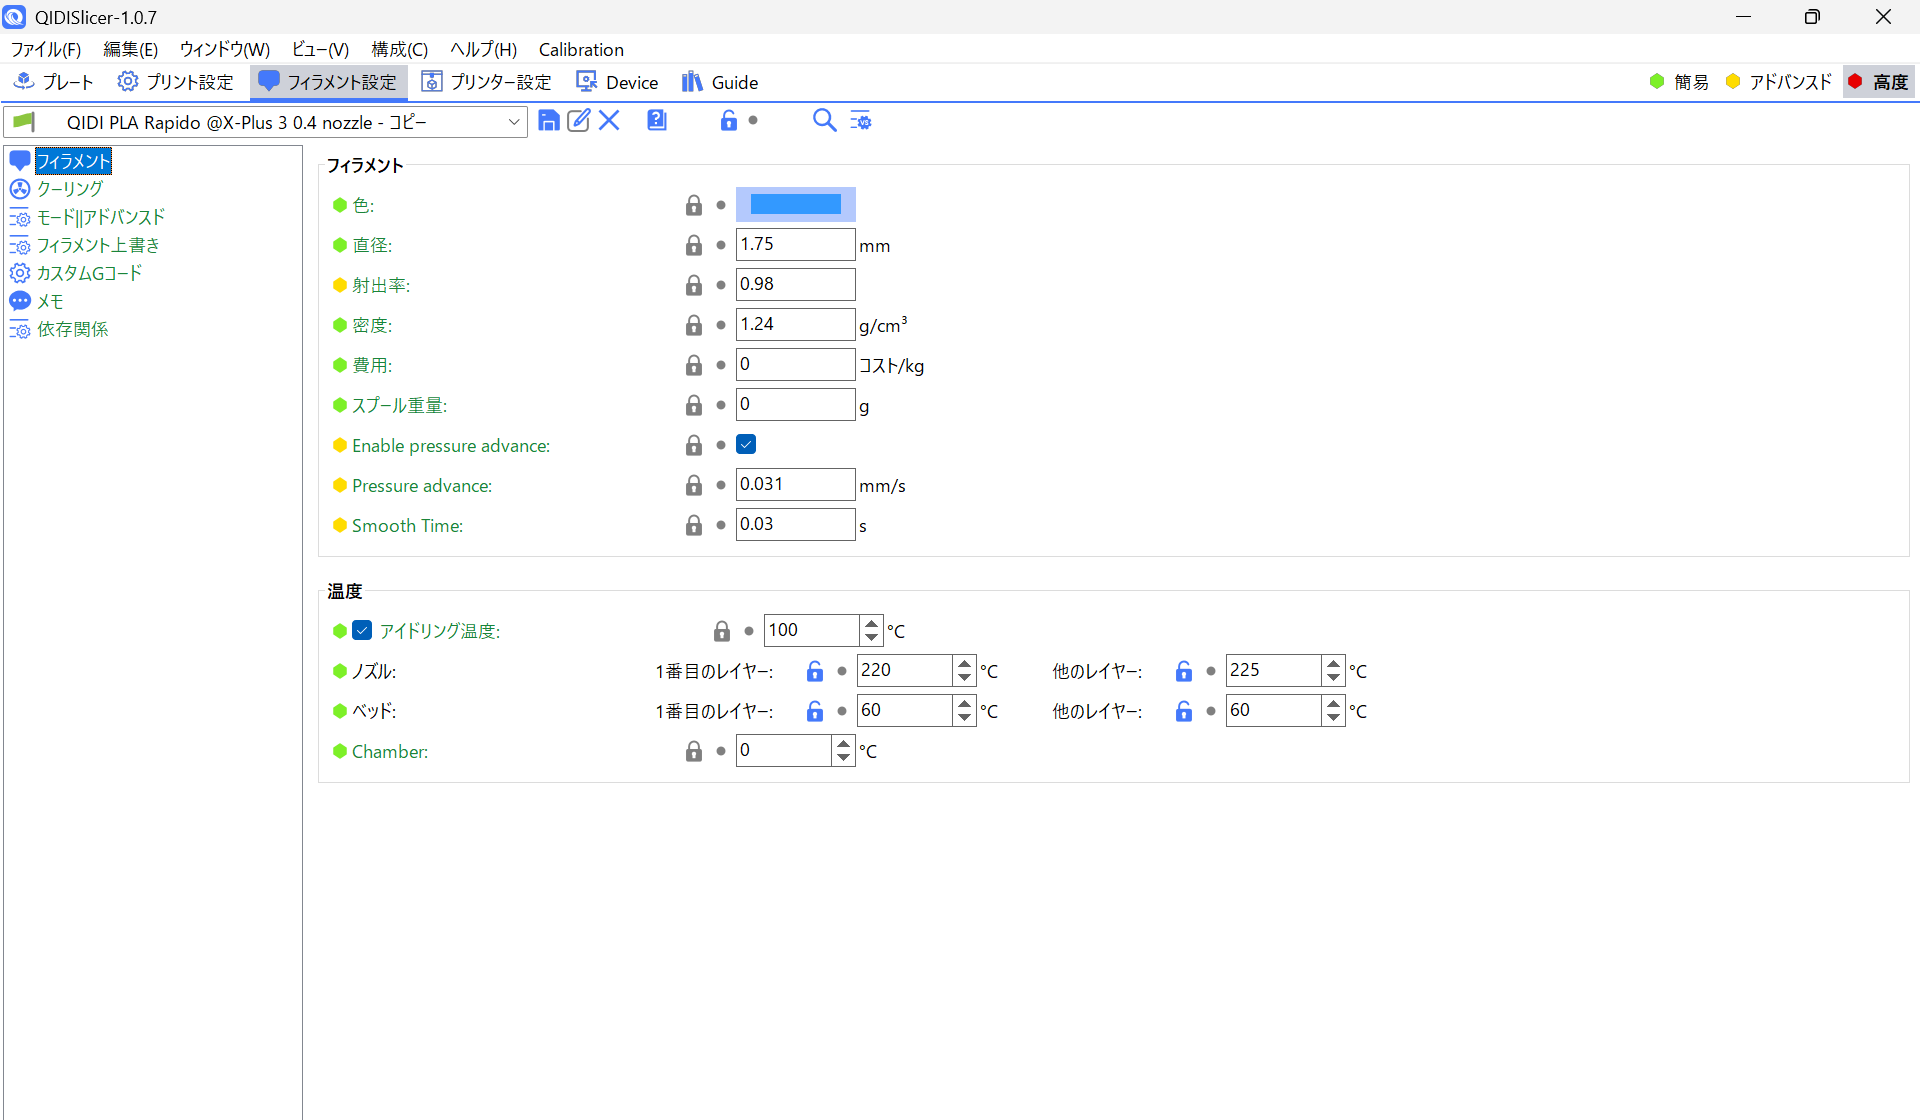
\includegraphics[scale=0.25]{./figure/設定4.png}
		\caption{フィラメント}
		\label{fig:slice4}
\end{figure}

\newpage

%%%%%%%%%%%%%%%%%%%%%%%%%%%%%%%%%%%%%%%%%%%%%%%%%%%%%%
\subsection{磁気トルカ駆動用のArduinoプログラム}
%%%%%%%%%%%%%%%%%%%%%%%%%%%%%%%%%%%%%%%%%%%%%%%%%%%%%%
 以下に,本研究で使用したArduino用のC++プログラムを示す.
\begin{lstlisting}
#include <Wire.h>
#include <SD.h>
#include <Adafruit_Sensor.h>
#include <Adafruit_BNO055.h>
#include <utility/imumaths.h>
#define PWM 9
#define VMAX 15.0f
#define RESISTER 18.37

bool flag = true;
double T=0.0327438; //実行時間
double e_pre = 0.0; // 微分の近似計算のための初期値
double de = 0.0; 
const int analogWriteStep = 255;
int dutyRatio = 80; //duty比[%]
double angle[3]={-1000,-1000,-1000};
double magne[3]={0,0,0};
double gyro[3]={-1000,-1000,-1000};
double bdot[3]={0,0,0};
double cross[3]={0,0,0};
double pre_gyro = 0;
unsigned long int time;
const int chipSelect = 10;
double kb = 0.00002;
double kp = 0.007;
double kd = 0.011;
double kc = 0.03;
double kw = 0.02;
double current = 0;
double voltage = 0;
double initmagne[3] = {0,0,0};
double normmag = 0;
double normmaginit = 0;
String datastr = "";
// Check I2C device address and correct line below (by default address is 0x29 or 0x28)
//                                   id, address
Adafruit_BNO055 bno = Adafruit_BNO055(55, 0x28, &Wire);

void setup(void)
{
  pinMode(10, OUTPUT);
  pinMode(9,OUTPUT);
  Serial.begin(115200);
  Serial.println("Orientation Sensor Test"); Serial.println("");
  //センサの初期化
  if (!bno.begin())
  {
    /* There was a problem detecting the BNO055 ... check your connections */
    Serial.print("Ooops, no BNO055 detected ... Check your wiring or I2C ADDR!");
    while (1);
  }
  //SDカードの初期化
  if (!SD.begin(chipSelect)) {
    Serial.println("SD card initialization failed!");
    while (1); // 初期化に失敗したら停止
  }
  Serial.println("initialization done.");
}

void loop(void){
  //could add VECTOR_ACCELEROMETER, VECTOR_MAGNETOMETER,VECTOR_GRAVITY...
  sensors_event_t orientationData , angVelocityData , linearAccelData, magnetometerData, accelerometerData, gravityData;
  bno.getEvent(&orientationData, Adafruit_BNO055::VECTOR_EULER);
  bno.getEvent(&angVelocityData, Adafruit_BNO055::VECTOR_GYROSCOPE);
  bno.getEvent(&linearAccelData, Adafruit_BNO055::VECTOR_LINEARACCEL);
  bno.getEvent(&magnetometerData, Adafruit_BNO055::VECTOR_MAGNETOMETER);
  bno.getEvent(&accelerometerData, Adafruit_BNO055::VECTOR_ACCELEROMETER);
  bno.getEvent(&gravityData, Adafruit_BNO055::VECTOR_GRAVITY);

  //センサの値を取得
  returnEvent(&orientationData,angle);
  returnEvent(&magnetometerData,magne);
  returnEvent(&angVelocityData,gyro);
  if(flag){
    for (int i = 0; i< 3; i++){
      initmagne[i]=magne[i];
    }
    normmaginit = sqrt(pow(magne[0],2)+pow(magne[1],2)+pow(magne[2],2));
    for (int i = 0; i< 3; i++){
      initmagne[i]=magne[i]/normmaginit;
    }
    flag = false;
  }
  //Bdot制御則の計算
  bdot[0]=magne[1]*gyro[2]-magne[2]*gyro[1];
  bdot[1]=magne[0]*gyro[2]-magne[2]*gyro[0];
  bdot[2]=magne[0]*gyro[1]-magne[1]*gyro[0];
  normmag = sqrt(pow(magne[0],2)+pow(magne[1],2)+pow(magne[2],2));
  cross[0]=initmagne[1]*(magne[2]/normmag)-initmagne[2]*(magne[1]/normmag);
  cross[1]=initmagne[0]*(magne[2]/normmag)-initmagne[2]*(magne[0]/normmag);
  cross[2]=initmagne[0]*(magne[1]/normmag)-initmagne[1]*(magne[0]/normmag);


  //目標角度を0[deg]とする
  double e = angle[0];
  if(e > 270){
    e = abs(e - 360);
  }
  de = (e - e_pre)/T;  

  //PD
  // current = kp*e + kd*de;
  //B-dot
  current = kb*bdot[0]/0.04935;
  // クロスプロダクト
  // current = (kc*cross[2] + kw*(gyro[2]-pre_gyro))/0.04935;

  //算出した電流値を電圧値に変換
  voltage = current * RESISTER;
  if(abs(voltage) > VMAX) {
    voltage = VMAX;
  }
  //電圧値をduty比に変換
  int duty = int(abs((voltage / 15.0) * 100.0));
  Serial.print(duty);

  int ledBrightness = analogWriteStep * duty / 100.0f;
  analogWrite( 9, ledBrightness );

  //値をstring型に
  datastr = String(angle[0]);
  for (int i = 0; i < 3; i++){
    datastr += ","+String(magne[i]);
  }
  datastr += ","+String(gyro[2]);
  //csvファイルのopen
  File angFile = SD.open("LOG.CSV", FILE_WRITE);
  //書き込み
  if (angFile) {
    angFile.println(datastr);
    angFile.close(); // ファイルを閉じる
    Serial.println("Write successful.");
  } else {
    Serial.println("Error opening test.txt for writing.");
  }
  e_pre = e;
  pre_gyro = gyro[2];
}

//センサの値を返す
void returnEvent(sensors_event_t* event,double tmp[3]) {
  double x = -1000000, y = -1000000 , z = -1000000; //dumb values, easy to spot problem
  else if (event->type == SENSOR_TYPE_ORIENTATION) {
    // Serial.print("orient:");
    x = event->orientation.x;
    y = event->orientation.y;
    z = event->orientation.z;
  }
  else if (event->type == SENSOR_TYPE_MAGNETIC_FIELD) {
    // Serial.print("Mag:");
    x = event->magnetic.x;
    y = event->magnetic.y;
    z = event->magnetic.z;
  }
  else if (event->type == SENSOR_TYPE_GYROSCOPE) {
    // Serial.print("Gyro:");
    x = event->gyro.x;
    y = event->gyro.y;
    z = event->gyro.z;
  }
  else if (event->type == SENSOR_TYPE_ROTATION_VECTOR) {
    Serial.print("Rot:");
    x = event->gyro.x;
    y = event->gyro.y;
    z = event->gyro.z;
  }
  else {
    Serial.print("Unk:");
  }
  tmp[0]=x;
  tmp[1]=y;
  tmp[2]=z;
}

  \end{lstlisting}

